% 2. RAG Entwicklung, welche Frameworks gibt es 
% -> Konfigurierbarkeit durch Files
% -> Maintainability
% -> Beliebtheit?
% -> Future Work (Haystack UI)
% -> Modularität (nach Gao.)
% -> IRA Methoden

\textcolor{blue}{Vielleicht nochmal neu sortieren: Vielleicht zur erst Evaluation und dann Fast-Rag Development into Transparency und Validity? Also Gedanklich von einem RAG Experiment into Viele RAG Experimente}

Developing retrieval-augmented generation systems is a difficult task that needs several reconfiguration phases.\cite{Simon.10112024} Component evaluation and in-depth failure analysis are key requirements for readjusting the right parts within the RAG-system, as they can include complex pipelines that may involve iterative or recursive processes. Failures can occur in many parts of the RAG-system. Barnett et al.\cite{Barnett.2024} created a list of 7 failures occuring in an advanced RAG system with Rewrite-Retrieve-Rerank-Read (4R) structure as Gao et al.\cite{Gao.18.12.2023} has defined it. Therefore for a framework it is indespensible to evaluate all components next to the end-to-end evaluation for the overall result. In this chapter, we will discuss how fast RAG development with transparent and reproducible results can be done. At first we will introduce Haystacks approach of fast RAG development. Secondly we will present classification metrics for end-to-end evaluation. Then we introduce failure types in RAG-systems and how to evaluate them. Lastly we will introduce the novelle blueprint by Simon et al.\cite{Simon.10112024} for handling external validity in RAG experiments. 

\section{Fast RAG Development}

\begin{figure}[b]
    \centering
    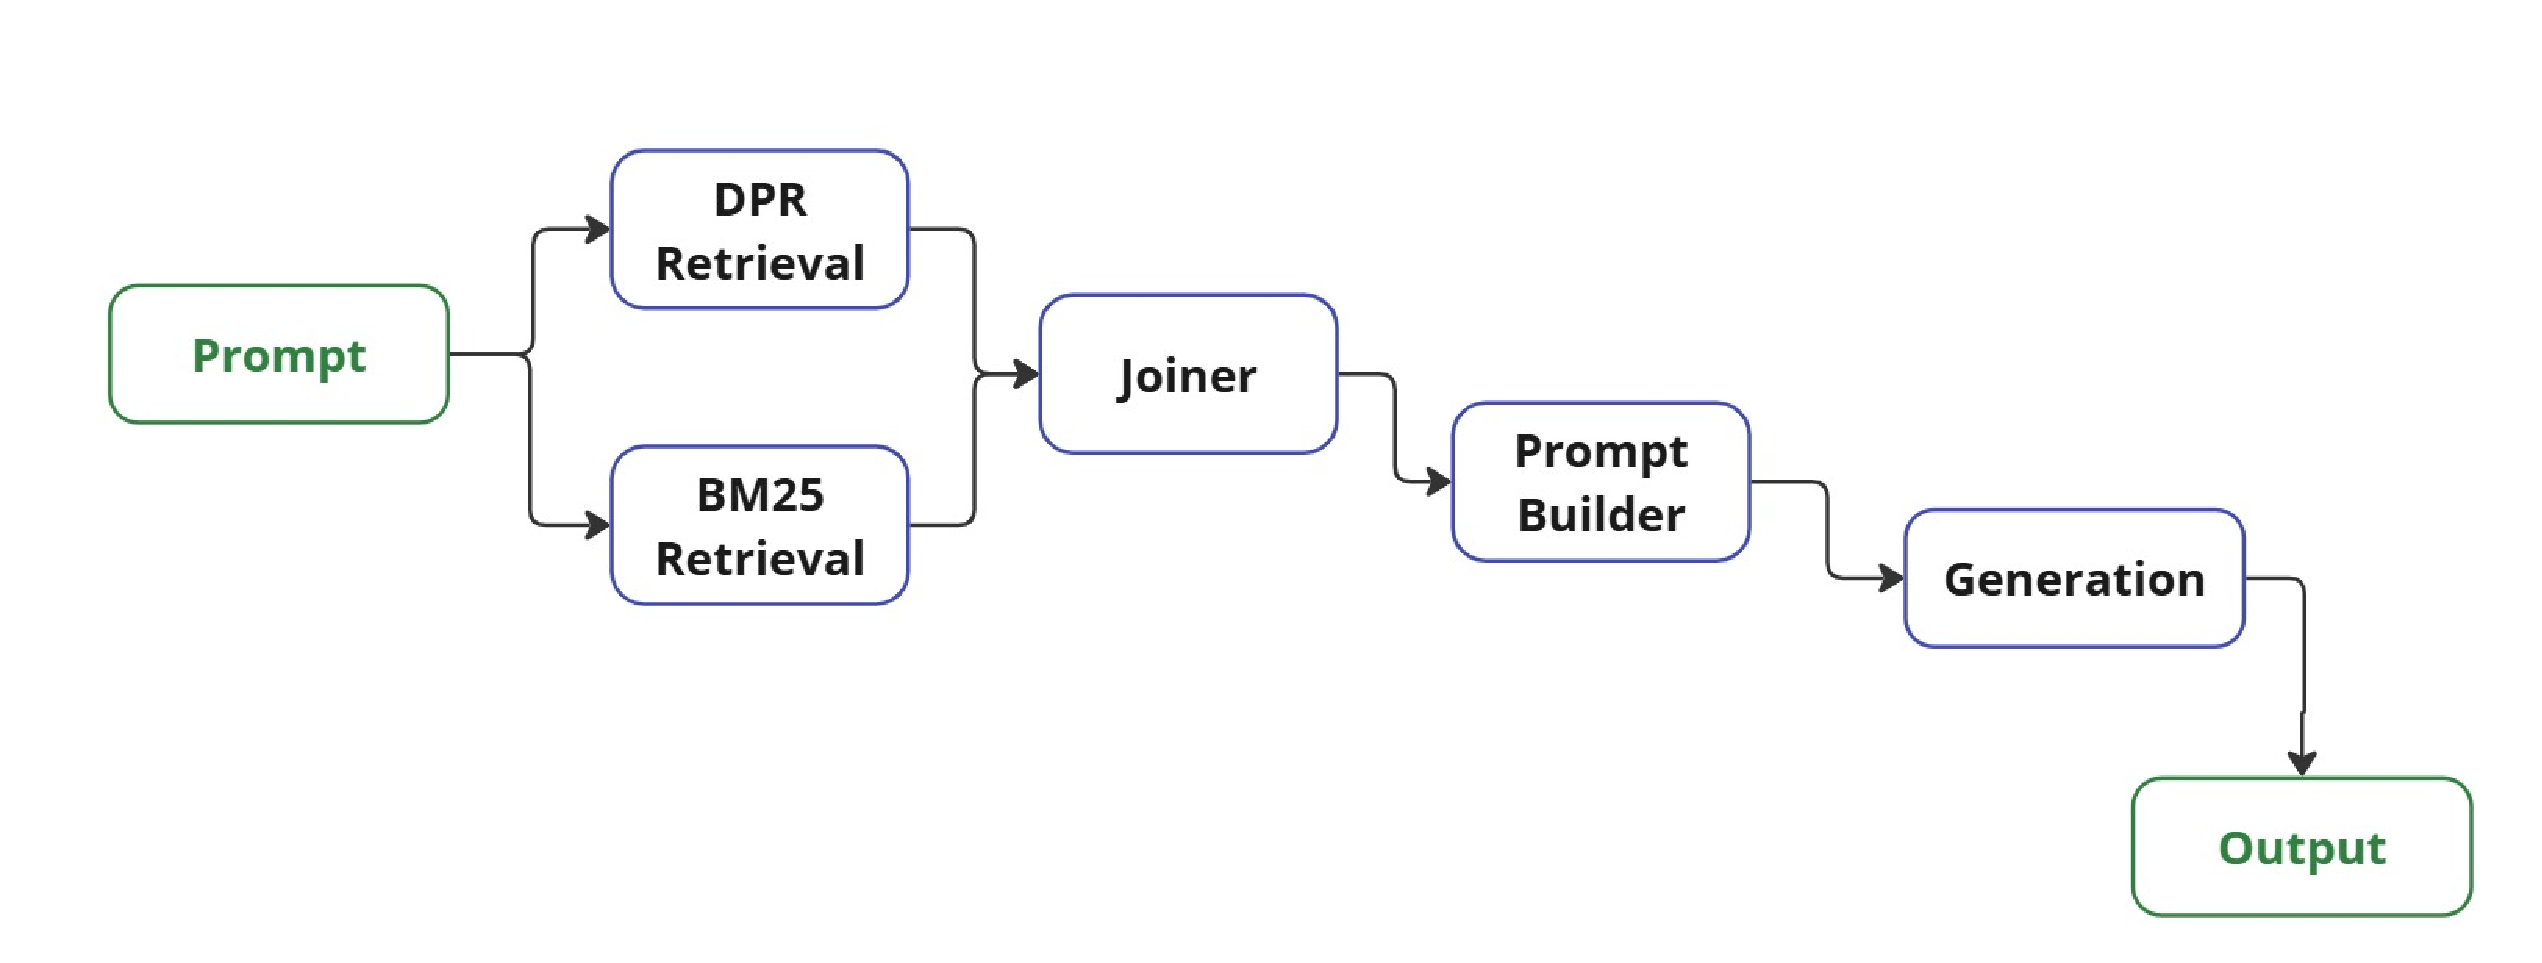
\includegraphics[width=\textwidth]{images/showcase-pipeline.pdf}
    \caption{A simple Retrieve-Read pipeline with both dense and sparse retrieval.}
    \label{fig:showcase}
\end{figure}


There are several RAG development tools and frameworks. Highly used ones are Llama-Index\cite{Liu_LlamaIndex_2022}, Langchain\cite{Chase_LangChain_2022} and Haystack\cite{Pietsch_Haystack_the_end-to-end_2019}. All of them offer comparable functionality for building advanced RAG systems in modularized architecture as introduced by Gao et al.\cite{Gao.18.12.2023}. Haystack does offer a functionality, where users can define a pipeline via a YAML-file. This enhances the reconfiguration of such systems, because instead of editing python files, there are just parameters in a YAML to be changed. This enhances the ability to report the methodologies of each experiment too. Instead of saving a python script or module for each configuration, only a YAML is stored that describes the tested RAG architecture fully. An example of this YAML definition can be seen in figure \ref{fig:showcase} and the YAML code below.

Furthermore Haystack comes with router components and the ability to create custom components, which enables iterative, recursive and adaptive RAG functionalities. Components in the Haystack universe can be seen as nodes of an RAG pipeline such as a generator or a retriever. 

\newpage
\begin{minted}[
    frame=single,
    bgcolor=lightgray
  ]{yaml}
components:
  llm:
    init_parameters:
      api_base_url: null
      api_key:
        env_vars: OPENAI_API_KEY
      ...
  prompt_builder: ...
  bm25_retriever: ...
  embedding_retriever: ...
  joiner: ...
  text_embedder: ...
  docs_embedder: ...
connections:
- receiver: llm.prompt
  sender: prompt_builder.prompt
- ...
\end{minted}

\textcolor{red}{Wie werde ich das nutzen? -> Umbauen für Matrix Angabe?}

\section{Evaluation Techniques}

Evaluating retrieval-augmented generation systems is a hard task that is still highly researched. It comes with all machine learning based evaluation problems such as data shifts, generalization errors or data contamination, but has also a variety of failure points introduced by the design of such a complex system. In this section I will introduce a majority of failure points for RAGs and present, how this framework helps to identify them. The final goal of tuning a RAG system is always to maximize its performance in end-to-end evaluation. RAG users want that the response of the systems fully answers its question or completes its task correct. Therefore end-to-end evaluation is important for comparing baselines and thus to decide if a RAG system can be a improvement to standalone large language models. 

\begin{figure}
  \centering
  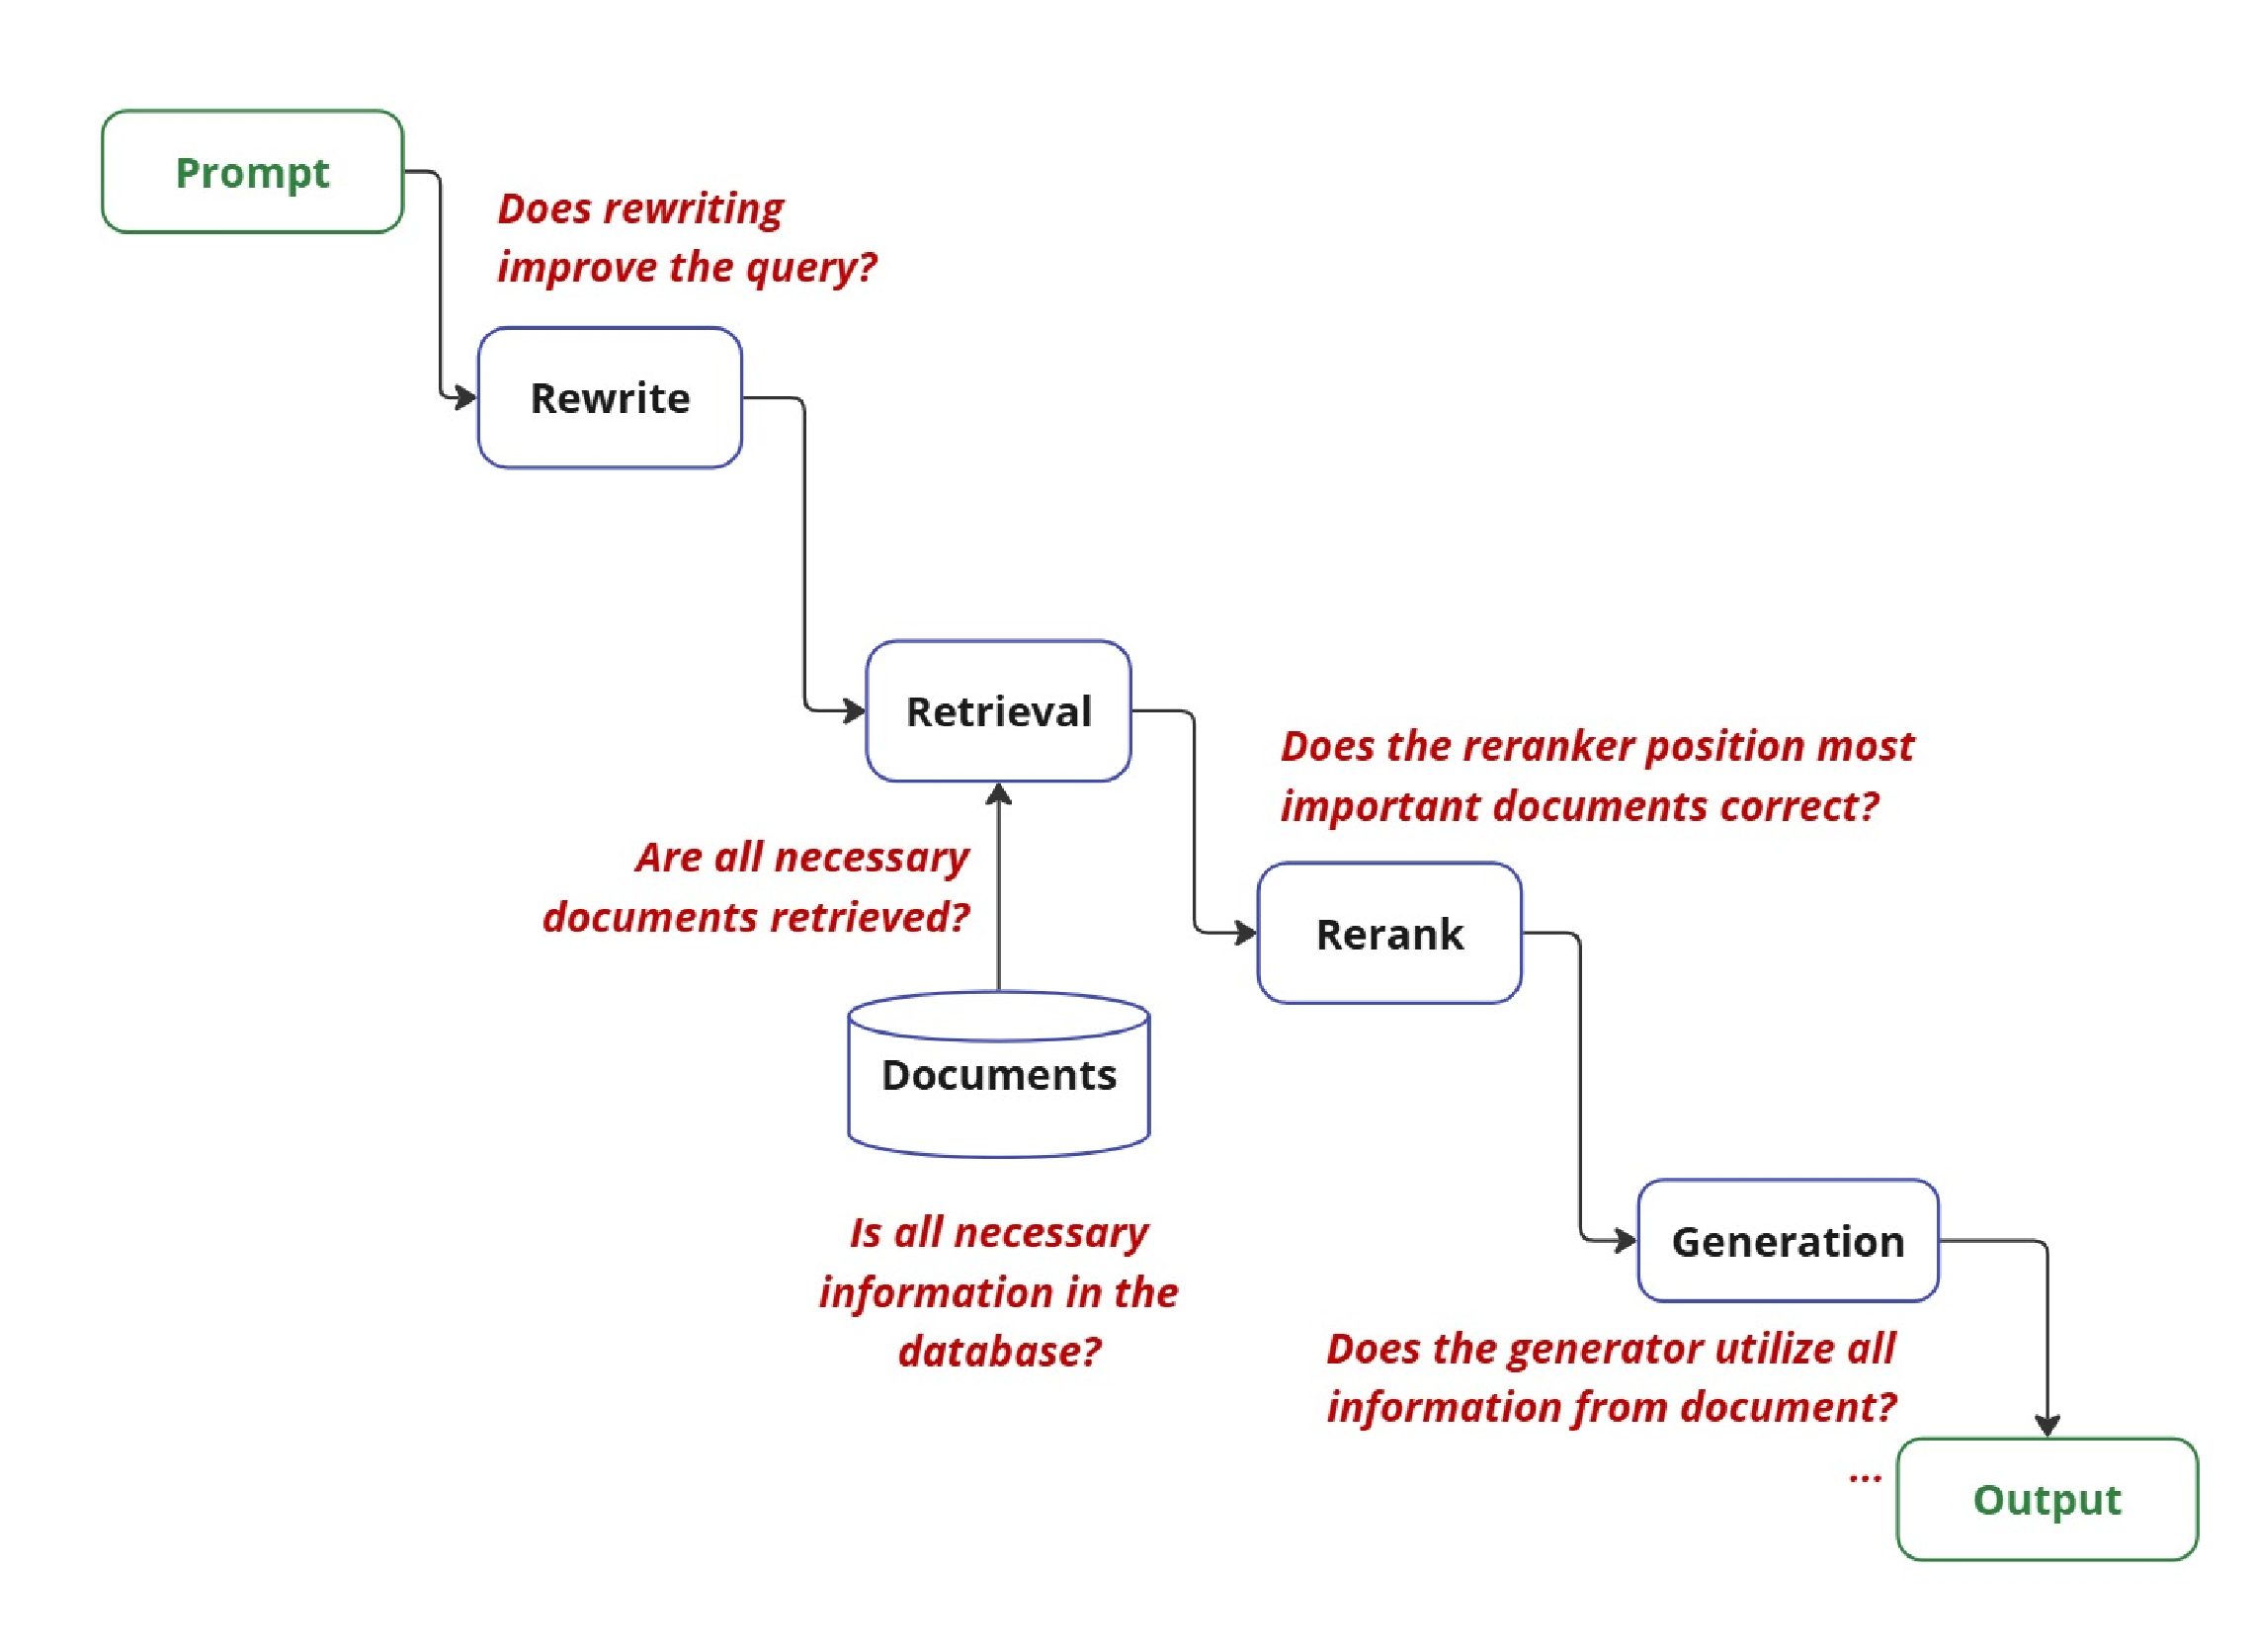
\includegraphics[width=\textwidth]{images/FailurePointExamples.pdf}
  \caption{A RAG pipeline with one failure example of all used components.}
  \label{fig:failures}
\end{figure}

The problem that occurs with end-to-end evaluation is that it is far from obvious which parameters we have to tune or which data we have to provide to accomplish a performance improvement. In figure \ref{fig:failures} there is an example for every component in particular RAG system. In reality there are much more points of failures in such systems. We will explore those in section component evaluation.

\subsection{End-to-End Evaluation}

We define end-to-end evaluation as metrics that use input and actual output to compare against a ground-truth output to decide if the evaluated item was correct or not. Evaluation that address retrieval are therefore not part of it. In this thesis we will focus on classification tasks only. Therefore the metrics we use for end-to-end evaluations are also limited by classification ones. 

{\renewcommand{\arraystretch}{1.5}%
\begin{table}
  \centering
 \begin{tabular}{|l|l|}
  \hline
  \textbf{Metric} & \textbf{Formula / Description} \\[3pt]
  \hline Accuracy & $\frac{TP + TN}{TP + TN + FP + FN}$\\[5pt]
  \hline Precision & $\frac{TP}{TP + FP}$\\[5pt]
  \hline Recall & $\frac{TP}{TP + FN}$\\[2pt]
  \hline F1-Score & $2 \times \frac{Precision \times Recall}{Precision + Recall}$\\[2pt]
  \hline Matthews Correlation & $\frac{TP \times TN - FP \times FN}{\sqrt{(TP + FP)(TP + FN)(TN + FP)(TN + FN)}}$\\Coefficient & \\[2pt]
  \hline False-Positive Rate & $\frac{FP}{FP + TN}$\\[2pt]
  \hline False-Negative Rate & $\frac{FN}{FN + TP}$\\[2pt]
  \hline Receiver Operating & Curve plotting TPR against FPR at various \\&threshold settings\\[2pt]
  \hline Area under ROC Curve &  AUC of the ROC curve\\[2pt]
  \hline pass@k & Probability of a correct solution in \textit{k} attempts \\[2pt]
  \hline
 \end{tabular}
 \caption{Typical classification metrics used for experiments including RAGs or LLMs\cite{Hou.8212023,Zeng.28.03.2024}}
 \label{table:classification_metrics}
\end{table}}

In stark contrast to evaluating generative tasks, classification comes with clear metrics or methods to evaluate outputs. In table \ref{table:classification_metrics} there is a list of highly used classification metrics for RAG and LLM experimentation.\cite{Hou.8212023,Zeng.28.03.2024} 

End-to-end evaluation requires the researcher to establish a baseline for the experiments. Baslines make experiment results interpretable and ensure that there is something to compare with. Therefore we decided to implement two baselines in this framework, which are used per default if an experiment starts. In the first run, we use the selected generator model alone to get a baseline vs standalone LLMs. Next we run a naive RAG with the data from the predefined corpus, the basic retrieval and generator (retrieve-read, cf: section \ref{sec:naive_rags}). The standalone LLM baseline ensure that the complexity overhead of implementing a RAG system is justified. If the evaluated RAG system can not surpass the performance of the LLM baseline, then simpler system should be used. Similar to that is the naive RAG baseline used to compare more complex RAG variations with more overhead, computation time or costs to the simpler naive one to ensure that the mentioned downsides are justified. We illustrated the prior defined state of our framework in figure \ref{fig:framework-baselines} to enhance the understanding of our considerations. The visualisation shows the process of reconfiguring the RAG system till its optimized towards a specific validation set. The reconfiguration phase can adjust parameters, using different models, pipelines or even fine-tuning parts such as retriever or generator. We will introduce detailed validity concerns of this common approach in a latter section.

\begin{figure}
  \centering
  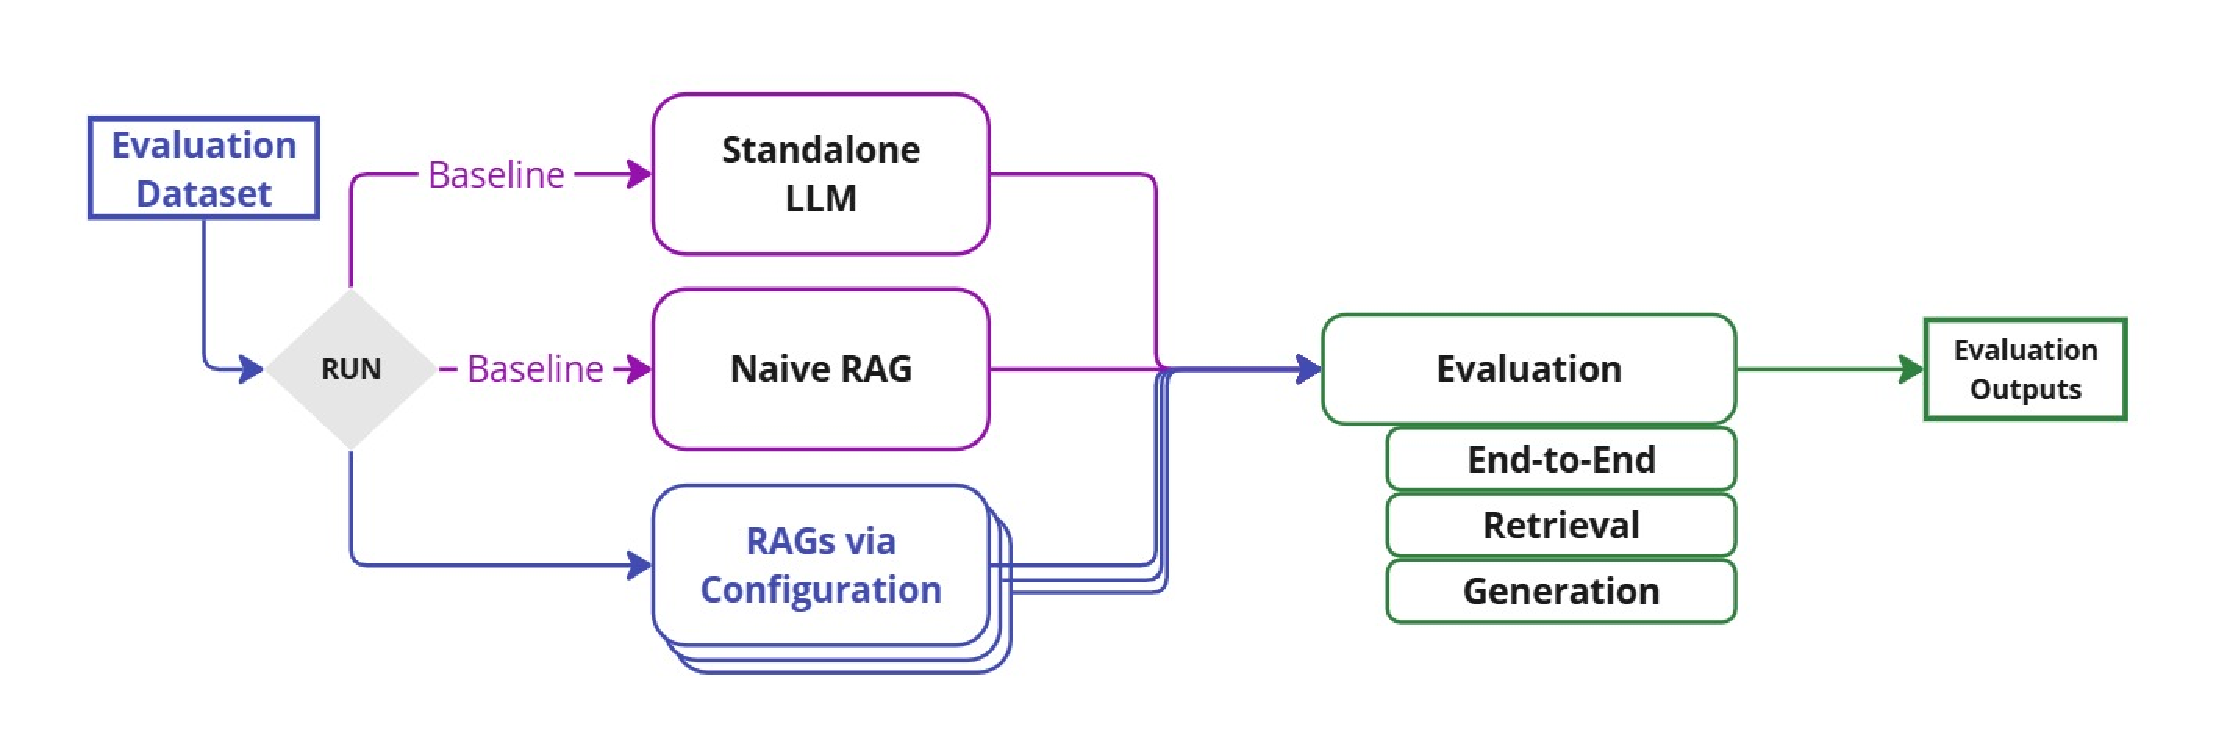
\includegraphics[width=\textwidth]{images/FrameworkBaselines.pdf}
  \caption{Framework: research define configuration files of RAG variations to evaluate them against the baselines standalone LLM and naive RAG with end-to-end evaluation.}
  \label{fig:framework-baselines}
\end{figure}

% \cite{Ru.15.08.2024.} Eventhough all components of a RAG-system affect its overall performance, there are ones that can not be evaluated directly.  \\


\subsection{Component Evaluation}

Component evaluation is necessary to detect performance issues of the whole systems introduced through individual components or pairs of components that are connected and do not work well together. In figure \ref{fig:failures}, we presented few of them. While this gives a good first impression of the variety of failures in a RAG system, this visualisation is far from complete. We argue that all components, no matter how small their impact is, can introduce significant failure rate for the overall system. Therefore it would be necessary to evaluate them all component-wise. We are not aware of papers that analyze component evaluation beside retrieval and read - the core components of a RAG system. Therefore we will introduce two new evaluations schemes to address all components in a advanced RAG system (4R, cf. section \ref{sec:advanced_rags}). Next to well studied topics retrieval evaluation and generation evaluation, we will implement rewrite evaluation and rerank evaluation. We will demonstrate the evaluation of all components while limiting ourself to the fixed advanced RAG definition (4R). We want to highlight here, that the modular RAG architecture with other components can be treated equally in this manner as long as there are metrics or evaluation techniques that can measure the performance of those components. The haystack library always returns inputs and outputs of each component to enable this kind of evaluation.

\paragraph{Rewrite}

Evaluating rewriter components is a derived task from the retrieval evaluation in the next section. The goal of rewriting is to transform the query so that the retriever finds all necessary documents or chunks for this task. One commonly used technique for that is \textit{Hypothetical Document Embeddings (HyDE)}\cite{Gao.2023}, next to query routing, query transformation and query expansion. Rewriter evaluation has the same metrics as the retriever, because it aims the same goals. The only difference in evaluating rewriters is, that instead of the retriever, the rewriter must be agnostic to replace them within the system. 

\textcolor{blue}{Wenn mir klar geworden ist, ob das praktisch umsetzbar ist (code it), dann sollte ich dafür hier eine Grafik einfügen.}

\textcolor{blue}{Eigentlich denke ich, dass auch Rewrite und Rerank isoliert evaluiert werden sollten. Notfalls mit LLM-as-a-Judge. Es ist eine methode es agnostisch zu machen, aber mMn wäre es präziser isoliert. (Hat wahrscheinlich Vor- und Nachteile. Isoliert $\longrightarrow$ präziser, Agnostisch mit Retrieval Metriken $\longrightarrow$ Synergy zwischen Rewriter und Retriever wird evaluiert.)}\textcolor{red}{Erstmal das offensichtliche machen - Retrieval und Generation Evaluation!}

\paragraph{Retrieve}
Retrieval Evaluation is possibly the most difficult part in the evaluation for several reasons. First, more retrieval do not imply better results and it is not clear nor obvious which set of documents perfectly serves the generator to give the best answer.\cite{Jin.5222024} Second, in a real world scenario indexed corpus, there are redundant and contradicting information.\cite{Yu.2024} Third, some questions or queries require to view the topic in a diverse manner, highlighting several considerations for different perspectives. Fourth, the quality of the query does affect the retrieval quality heavily, because queries can be too complex and ambigious or not even requiring retrieval, which may also lead to LLM hallucinations.\cite{Huang.2023}



\paragraph{Rerank}


\begin{itemize}
    \item 7 Failures
    \item How to Evaluate those
\end{itemize}

\paragraph{Generators}
Generators are based on transformer architecture and classification tasks were not the initial intention for this kind of tasks. Thus it is important that outputs are in a wanted form such as "valid", or "invalid".

\subsection{Component Block Evaluation}
\textcolor{blue}{Finde das Paper, in dem gesagt wurde, dass verschiedene Retrievals mit verschiedenen Generators gut zusammenarbeiten, (auch vorstellbar Retriever (Sparse vs Dense) mit verschiedenen Rewritern)}

\begin{figure}
  \centering
  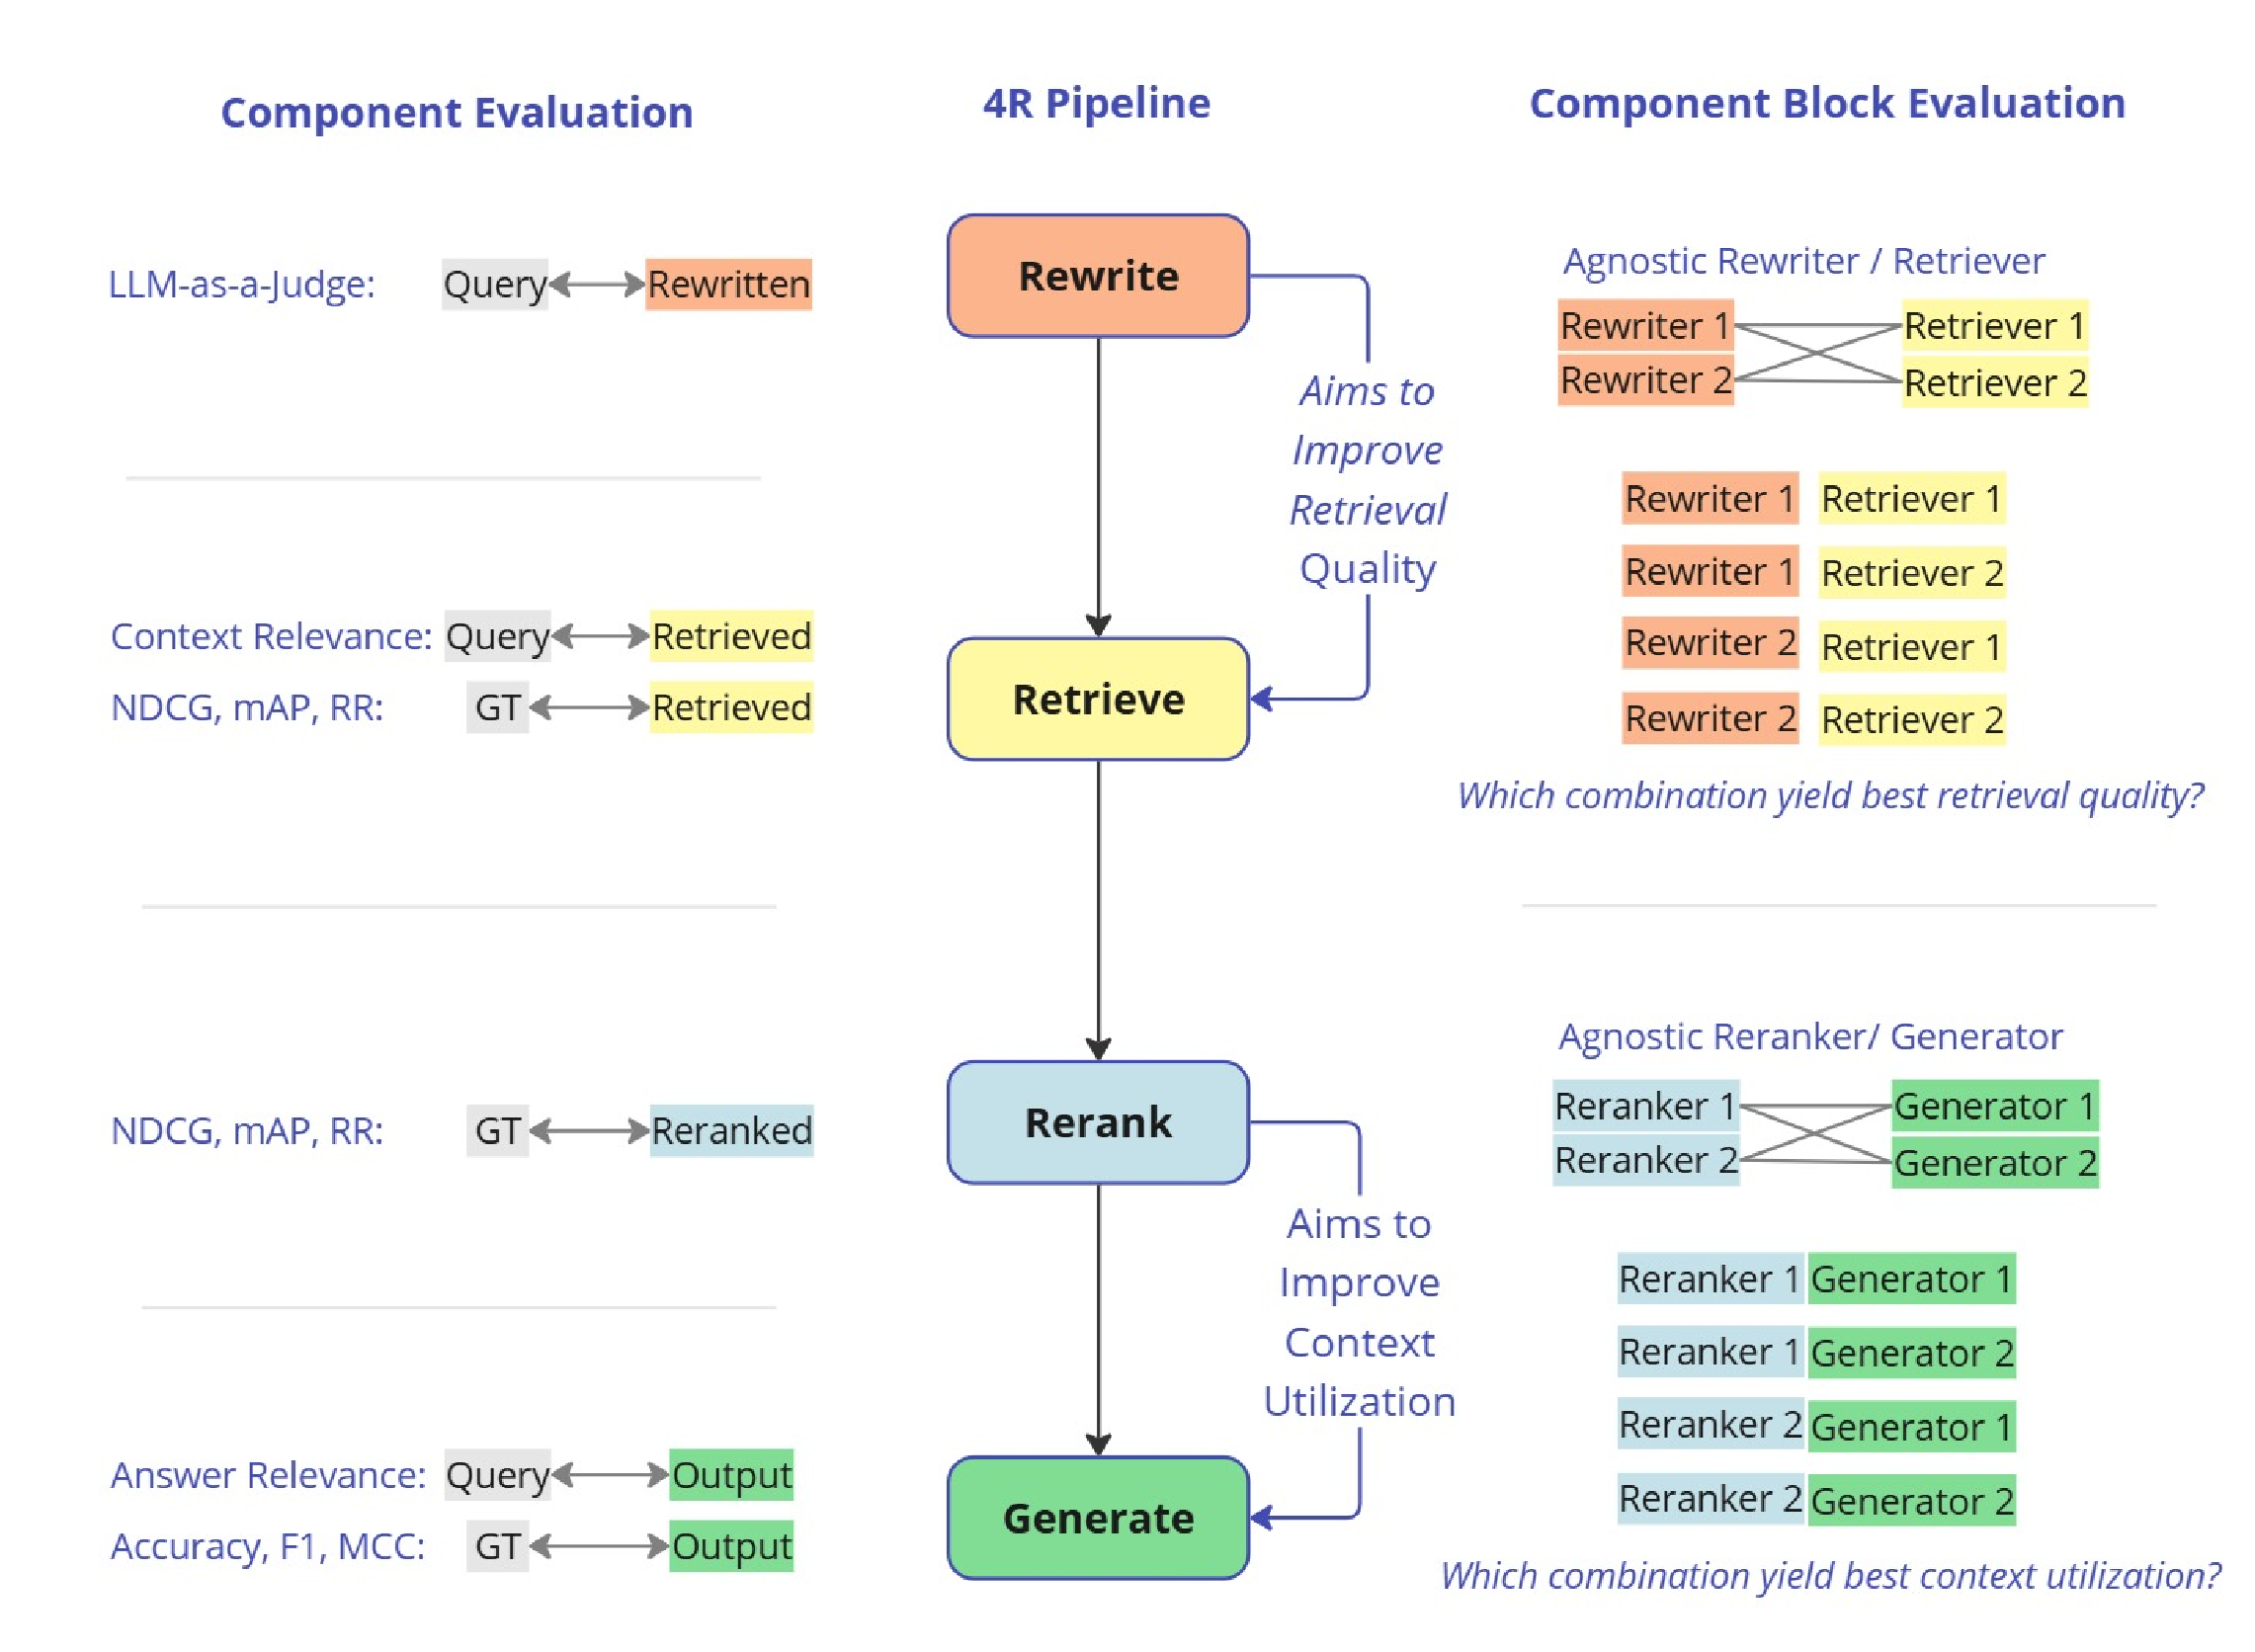
\includegraphics[width=\textwidth]{images/ComponentBlockEvaluation.pdf}
  \caption{Comparison of isolated component evaluation of each component and component block evaluation, where several components with the same goal are evaluated.}
  \label{fig:componentblockeval}
\end{figure}

\section{Increasing Transparency in RAG Experiments}

\begin{itemize}
    \item DVC for RAG Experiments
    \item Save YAMLs, Versionize Data + Code
\end{itemize}

\section{External Validity of RAG Experiments}

\begin{figure}
    \centering
    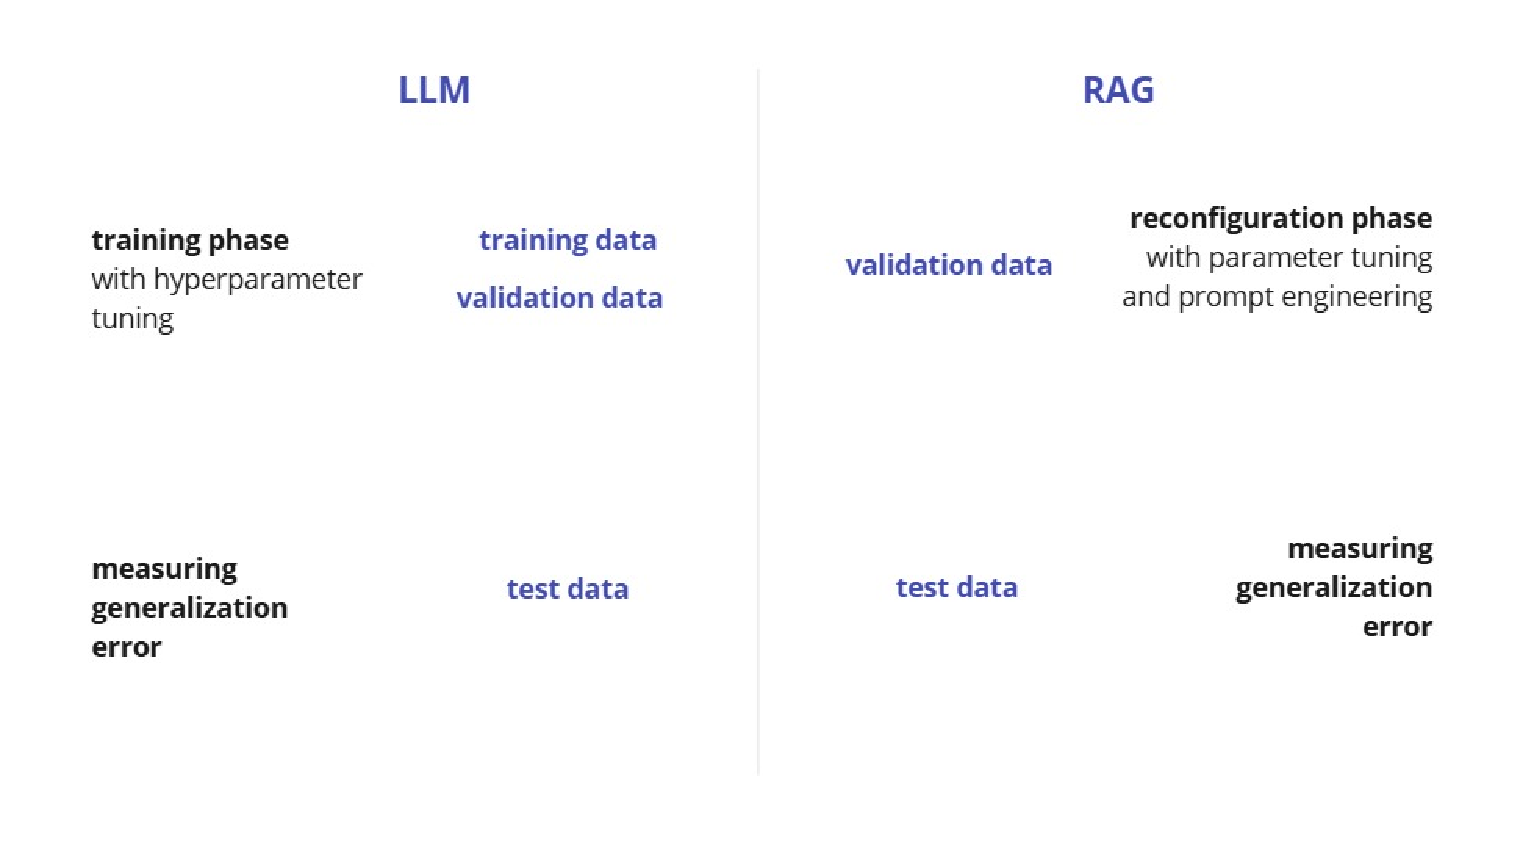
\includegraphics[width=\textwidth]{images/RAGvsLLM-tuning.pdf}
    \caption{Comparison of reconfiguration between RAGs and LLMs - both relying on tuning parameters and test data.}
    \label{fig:tuning}
\end{figure}


Data is rare, especially for down-stream tasks in domains such as configuration validation or similar tasks. They often rely on few datasets that can not represent the whole domain. Therefore there are measures required to ensure that the developed systems can be generalized from the seen data to the unseen production data. Measuring generalization error in the large language model development is done by splitting the data into training, validation and test datasets. While the training and validation data is used for hyperparameter tuning to ensure the best performing model, the test dataset on the other hand is used to check if the hyperparameter tuning introduced an overfitting. This procedure must be adopted for RAG systems too (cf. figure \ref{fig:tuning}). Even though they do not rely on a training in the most cases, the continous reconfiguration of such systems, including prompt engineering or parameter tuning can lead to differences in seen and unseen data. The needs for a test dataset is independent from a potential training phase, but instead very dependent on a tuning phase for the systems, that is done till the results converge to the best outcoming scenario. Both LLM and RAG development share those reconfiguration phases. 

\textcolor{blue}{Selbst wenn tuning RAGs nicht super anfällig für Overfitting sein sollten, gibt es ja fine-tuning für Retrieval, Generators und Co., welche Overfitting einführen können. Diese werden dann mit dem Objective im RAG bestmöglich zu performen trainiert, daher muss auch da der Generalization Error überprüft werden.}

\paragraph{RAG Evaluation needs a Holdout-Testset}
\begin{itemize}
    \item RAG Experiments belongs to ML Experiments 
    \item Requires Seeding
    \item ML Experiments might cause Overfitting
    \item Generalization (External Validity) is testable with a hard data split (train vs validation vs test)
    \item training data split is not needed, but validation and test is required
    \item validation is for hyperparameter tuning important, which configs have the best results
    \item no testset -> no generalization estimatation
    \item \textcolor{red}{Problem zum Nachdenken} Im Training braucht es ein Holdout-Testset damit man das LLM auswählen kann, welches den geringsten Testfehler hat, aber im RAG wird nicht trainiert. Müssen dann alle Konfigurationen dagegen getestet werden?
\end{itemize}


\section{CLI}

\begin{figure}[!ht]
    \centering
    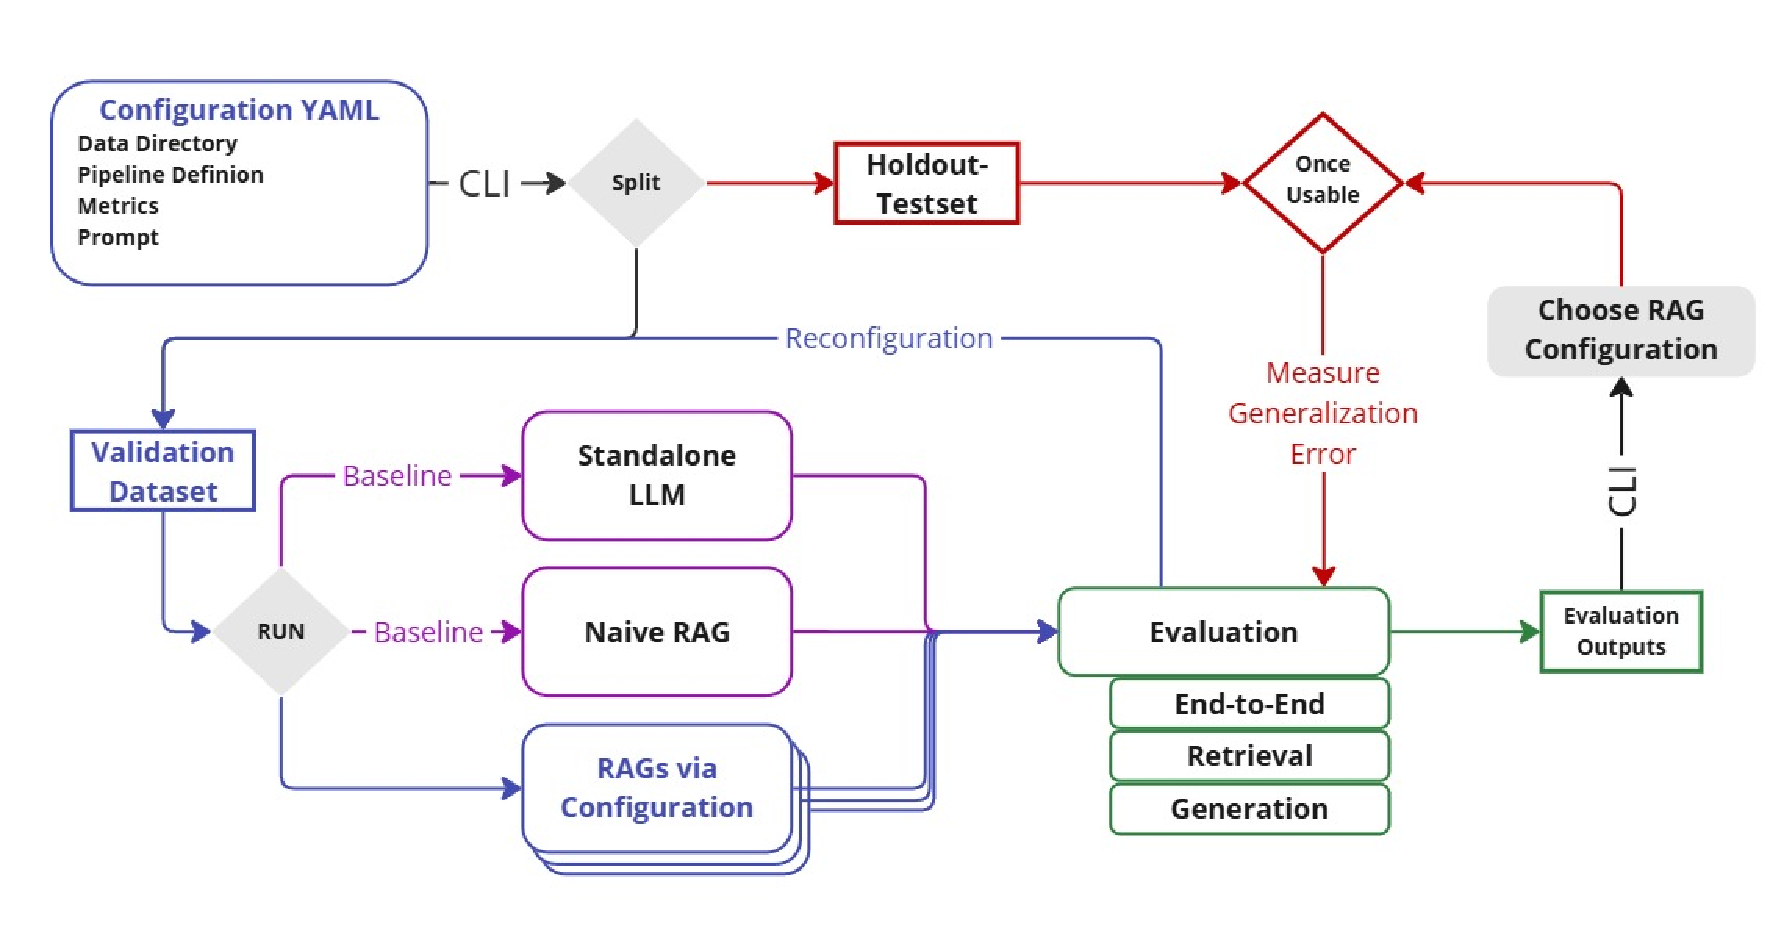
\includegraphics[width=\textwidth]{images/Sketch.pdf}
    \caption{...}
    \label{fig:EvaluationDesign}
\end{figure}

We use the presented Haystack functionalities to build a CLI-based framework around it. Our complete appraoch can be seen in figure \ref{fig:EvaluationDesign}. Given a data directory, pipeline and metrics definition, we first split the data into a validation and holdout-test dataset based on a split parameter \textit{test\_size}. Next we use the resulting validation dataset to run the first evaluations on the data. For that it loads the pipeline and data from its paths and starts with evaluating against a standalone LLM to have a baseline if RAG at all is a significant improvement in contrast to having just an LLM. Next, it ingests data into a vector database and builds an naive RAG with (Retrieve-Read) architecture as another baseline in contast to the in the YAML file defined advanced RAG architecture. The same procedure starts with the RAG configuration from the file. Each run gets evaluated in respect to End-to-End evaluation and component-wise. Evaluations are visualized in \textcolor{red}{EVAL INFOS EINFÜGEN Framework oder PRozess für Indepth Failure Analysis hier erklären}. After failure analysis, the RAG can be reconfigured again to test new parameters. 

\textcolor{blue}{Here comes text how to use Holdout-Test dataset}



\section{Limitations}

List of possible Limitations

\begin{itemize}
    \item Generation Tasks 
    \item Chunking Reconfiguration
\end{itemize}